% PROVENANCE (section-level)
%   status      : CODE_FACT
%   produced-by : 4_LightGBM_Multiclass_Training.py (hyper-parameters,
%                 schedule); BDTs/LightGBM/eval_result_v{1,2,3}.json (metrics);
%                 BDTs/LightGBM/lgbm_multiclass_v3.txt (model header)
%   commit      : ad2f2ec
%   sample      : MC16rd training sample, e and mu
%   selection   : offline_cut (Eq. offline-cut)
%   corrections : none applied at training time
\section{BDT Training and Validation}
\label{app:mva}

\begin{table}[htbp]
  \centering
  \caption{LightGBM configuration of the four-class classifier, hard-coded in
  \texttt{4\_LightGBM\_Multiclass\_Training.py} at commit \texttt{ad2f2ec}.}
  \label{tab:mva-hyperparameters}
  \small
  \begin{tabular}{l l l}
    \hline
    Parameter & Value & Role \\
    \hline
    \texttt{boosting\_type} & \texttt{gbdt} & gradient boosted trees \\
    \texttt{objective} & \texttt{multiclass}, \texttt{num\_class} 4 & four-class output \\
    \texttt{metric} & \texttt{multi\_logloss}, \texttt{auc\_mu} & monitored each round \\
    \texttt{learning\_rate} & 0.5, then $0.5 \times 0.99^{i}$ & large, then decaying \\
    \texttt{num\_boost\_round} & 15 then 10 & two stages \\
    \texttt{early\_stopping} & 3 then 2 rounds & per stage \\
    \texttt{num\_leaves} & 49 & tree capacity \\
    \texttt{min\_child\_samples} & 1000 & leaf occupancy floor \\
    \texttt{bagging\_fraction} & 0.7, \texttt{bagging\_freq} 5 & row subsampling \\
    \texttt{feature\_fraction} & 0.7 & column subsampling \\
    \texttt{lambda\_l1}, \texttt{lambda\_l2} & 1, 1 & regularization \\
    \texttt{seed} & 0 & reproducibility \\
    \hline
  \end{tabular}
\end{table}

We use a BDT with \texttt{min\_child\_samples} $=1000$ and only 49 leaves,
and 25 boosting rounds. This gives a small and regularized model.

We use separate training and validation samples. We find no evidence for over-training of the BDT.



\subsection{BDT Input variables}
\label{app:mva:inputs}

The BDT uses 17 input features, which are listed in 
Appendix~\ref{app:selections:mva}. The variables excluded from training are given 
in Appendix~\ref{app:selections:excluded}.

% PROVENANCE
%   status      : PRELIMINARY_RESULT
%   produced-by : utilities.apply_mva_bcs() (importance=True branch,
%                 lgb.plot_importance(..., importance_type='gain')); the
%                 calling notebook/script was not identified
%   commit      : ad2f2ec
%   sample      : MC16rd BDT training sample (Sec.~\ref{sec:mva:classes})
%   selection   : offline_cut (Eq. offline-cut); model version not confirmed
%   corrections : none applied at training time
\begin{figure}[htbp]
  \centering
  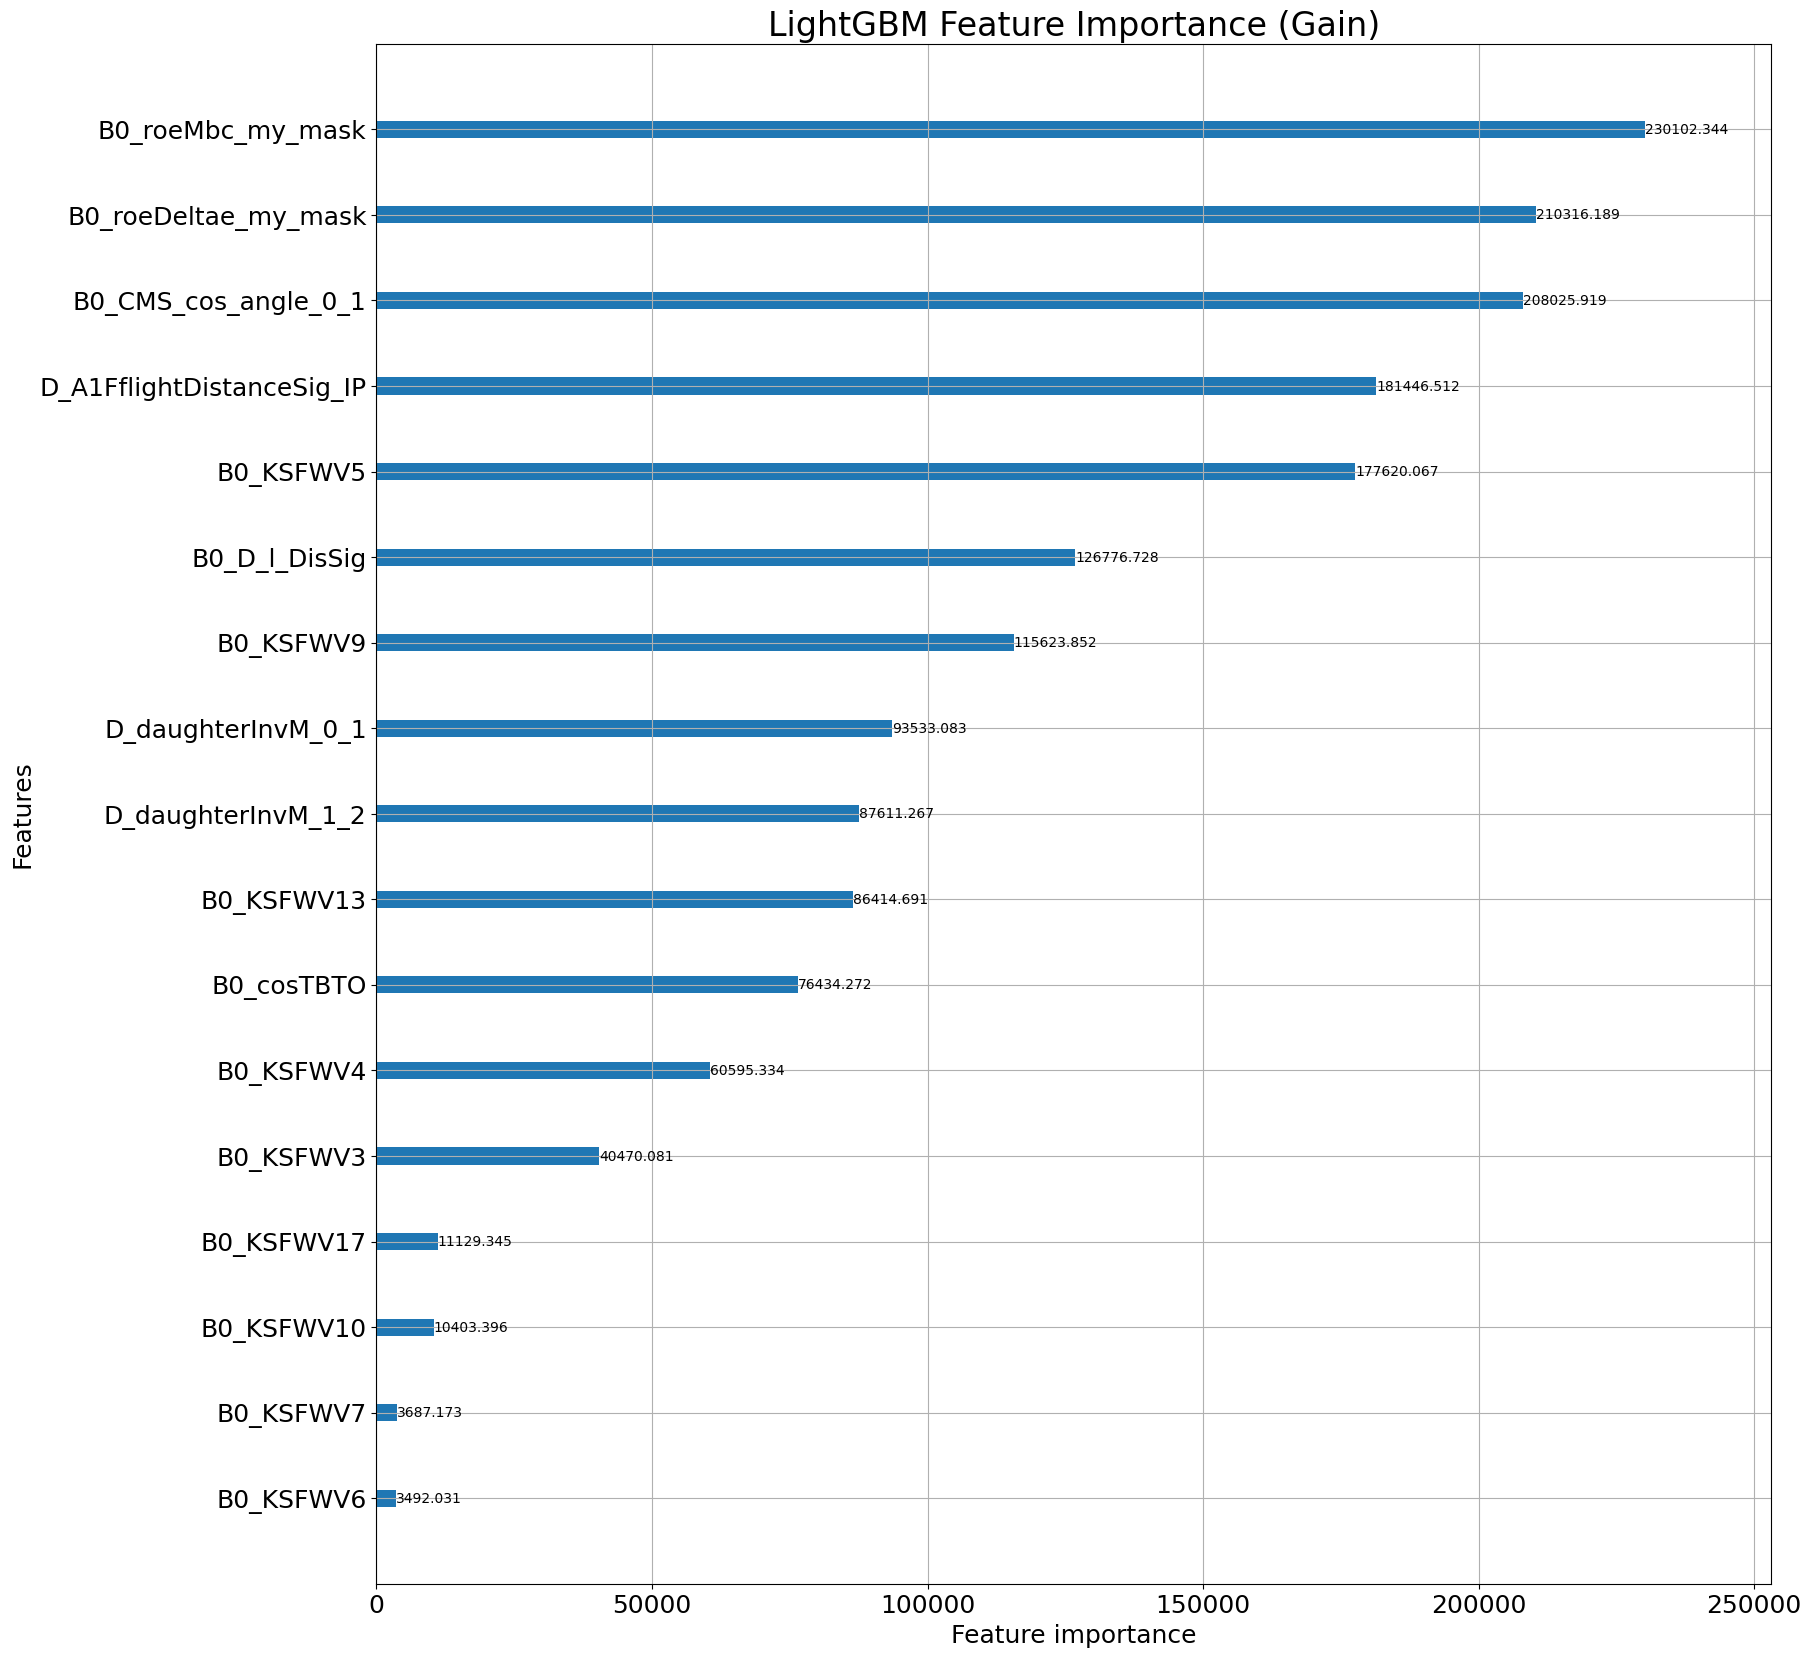
\includegraphics[width=0.85\textwidth]{LGBM_feature_importance.png}
  \caption{LightGBM feature importance (total split gain) for the 17 training
  variables of Appendix~\ref{app:selections:mva}.
  The two ROE kinematic variables ($M_{\mathrm{bc}}^{\mathrm{ROE}}$,
  $\Delta E^{\mathrm{ROE}}$) and $B_0\_CMS\_cos\_angle\_0\_1$ dominate;
  \texttt{D\_A1FflightDistanceSig\_IP}, the $D$ flight-distance significance
  of Sec.~\ref{sec:recon:d}, is the next most important, ahead of any single
  continuum-suppression variable.}
  
  \label{fig:lgbm-importance}
\end{figure}

\subsection{Additional Information on the BDT Classifier to be added}
\label{app:mva:todo}

\AnalysisTBD{ROC or efficiency-versus-purity curves for each of the four
classes on the validation subset}
\AnalysisTBD{learning curves per round, from the stored evaluation histories}
\AnalysisTBD{distributions of every retained input variable, data versus
simulation, in an unblinded control region}
